\section{Versuchsaufbau und Durchf"uhrung} % (fold)
\label{sec:durchf_uhrung}

\subsection{Versuchsaufbau} % (fold)
\label{sub:aufbau}

\begin{figure}[!h]
	\centering
	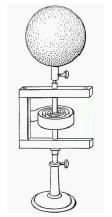
\includegraphics[width = 2cm]{img/Drillachse.PNG}
	\caption{Drillachse mit eingespannter Kugel. \cite{anleitung}}
	\label{drillachse}
\end{figure}

Bei dem Versuch zur Bestimmung des Tr"agheitsmoments $I$ von verschiedenen K"orpern wird eine Drillachse verwendet \ref{drillachse}. Diese besteht aus einer zweifach im Raum drehbar gelagerten Achse, welche "uber eine Spiralfeder mit dem Rahmen verbunden ist.
Auf diese Achse k"onnen die verschiedenen K"orper befestigt werden.

\subsection{Durchf"uhrung} % (fold)
\label{sub:durchf_uhrung}

\subsubsection{Statische Methode} % (fold)
\label{sub:statische_methode}

Ein Metallstab wird symmetrisch auf die Drillachse geschraubt. 
Mithilfe einer Federwaage wird die r"ucktreibende Kraft gemessen, die bei dem Auslenkwinkel $\varphi$ wirkt.
Dabei muss die Federwaage senkrecht zum Radius der vom K"orper beschriebenen Kreisbahn gehalten werden.

Nun kann die Winkelrichtgr"o"se $D$ aus der Federkraft $F$, dem Abstand $r$ zur Drehachse und dem Drehwinkel $\varphi$ bestimmt werden:

\begin{equation}
 	D = \frac{F \cdot r}{\varphi} \qquad .
\end{equation} 

Diese Messung wird f"ur 10 verschiedene Auslenkwinkel durchgef"uhrt.

\subsubsection{Dynamische Methode} % (fold)
\label{sub:dynamische_methode}
 
Eine Metallstange mit Gewichten an den Enden wird symmetrisch auf die Drillachse geschraubt. Das System wird in Schwingung versetzt und die Schwingungsdauer $T$ gemessen. Diese Messung wird f"ur 10 verschiedene Abst"ande der Massen zur Drehachse wiederholt.

\subsubsection{Messung des Tr"agheitsmoments eines K"orpers} % (fold)
\label{sub:tr_agheitsmoment_verschiedener_k_orper}

Auf die Drillachse wird ein K"orper geschraubt.
Die Schwingungsdauer $T$ wird gemessen.
Diese Messung wird 5 mal wiederholt f"ur zwei verschiedene K"orper.

\subsubsection{Messung des Tr"agheitsmoments einer Puppe} % (fold)
\label{sub:messung_des_tr_agheitsmoments_einer_puppe}

Eine Holzpuppe wird auf die Drillachse geschraubt.
Es wird 5 mal die Schwingungsdauer $T$ gemessen.
Dies wird f"ur insgesamt zwei K"orperhaltungen wiederholt.
Die Puppe wird Ausgemessen, damit man eine gute N"aherung des K"orpers als zusammensetzung mehrerer Zylinder erh"alt.

\subsection{Bestimmung des Tr"agheitsmoments eines Menschen} % (fold)
\label{sub:bestimmung_des_tr_agheitsmoments_eines_menschen}

Der K"orper eines Menschen wird vermessen um aus Zylindern bestehend gen"ahert werden zu k"onnen. Daraus wird das Tr"agheitsmoment eines Menschen abgesch"atzt.